\cleardoublepage % memastikan bab baru dimulai di halaman ganjil (kanan)
\chapter{STUDI LITERATUR}
\label{chap:studi-literatur}
\section{Olahraga Lari \textit{Ultra-marathon}}
\textit{Ultra-marathon} adalah cabang olahraga lari jarak jauh yang menempuh jarak lebih dari jarak maraton pada umumnya, yaitu sepanjang 42,195 kilometer. \textit{Event ultra-marathon} dapat berupa lari dengan jarak tetap misalnya 50 km, 100 km, atau lebih. Selain itu, dapat juga berbasis pada waktu, misalnya 6 jam, 12 jam, atau 24 jam, di mana pelari menempuh jarak sejauh mungkin dalam waktu yang ditentukan \cite{scheer2020defining}. \textit{Ultra-marathon} sendiri menuntut pelari memiliki ketahanan fisik dan mental yang luar biasa, serta memerlukan strategi \textit{pacing} dan manajemen energi yang tepat selama kompetisi berlangsung.

Berbeda dengan maraton biasanya, \textit{ultra-marathon} sering kali melibatkan medan yang lebih menantang seperti gunung, \textit{trail}, atau kombinasi berbagai jenis permukaan. Faktor lingkungan seperti elevasi lintasan, cuaca ekstrem, dan durasi kegiatan yang panjang menjadikan aspek keselamatan dan pelacakan peserta sebagai prioritas utama dalam penyelenggaraan kegiatan ini \cite{hoffman2011factors}.
Oleh karena itu, sistem pendukung untuk komunikasi dan pelacakan menjadi sesuatu yang diperlukan dalam operasional \textit{ultra-marathon}. Kebutuhan ini tidak hanya terbatas pada panitia dan peserta, tetapi juga dibutuhkan oleh tim support dan penonton  agar dapat memantau dan memberikan dukungan secara tepat dan efisien sepanjang kegiatan \textit{Ultra-Maraton} berlangsung.

\section{ITB Ultra-Marathon}
ITB Ultra-Marathon adalah \textit{event} lari jarak ultra yang diselenggarakan oleh Komisariat ITB Ultra dan Ikatan Alumni Institut Teknologi Bandung. Kegiatan ini pertama kali diadakan pada tahun 2017 dan telah menjadi ajang tahunan yang menarik perhatian pelari dari berbagai kalangan \cite{Hafizh2025}. ITB Ultra-Marathon diinisiasi bersama oleh ITB dan Yayasan Solidarity Forever, acara ini konsisten memperkuat ikatan antara sivitas akademika, alumni, beserta keluarga. \textit{Event} ini juga menjadi simbol kontribusi ITB dalam memajukan olahraga daya tahan (\textit{endurance sport}) serta menyuarakan nilai persatuan dalam keberagaman. Berbeda dengan maraton pada umumnya, \textit{event} ini menempuh jarak yang jauh lebih panjang, yaitu sepanjang 180 kilometer, dengan rute yang menantang dari Jakarta dan berakhir di Kampus Ganesha ITB, Bandung.

Gambar \ref{fig:rute-itb-ultra-2025} merupakan visualisasi rute ITB Ultra-Marathon 2025 yang membentang dari Jakarta menuju Kampus Ganesha ITB, Bandung. Rute sepanjang sekitar 180 kilometer ini melewati berbagai kota dan wilayah seperti Jakarta, Bogor, Puncak, Cianjur, Padalarang, dan Cimahi sebelum akhirnya memasuki Kota Bandung. Setiap titik penanda pada peta menunjukkan lokasi-lokasi penting yang dilewati oleh peserta, yang mencerminkan karakteristik rute yang beragam mulai dari kawasan perkotaan, perbukitan, hingga area pegunungan. Visualisasi ini memberikan gambaran menyeluruh mengenai kompleksitas medan yang harus dilalui serta menegaskan tantangan fisik yang dihadapi pelari dalam ajang \textit{ultra-marathon} ini.
\begin{figure}[H]
    \centering
    \captionsetup{justification=centering}
    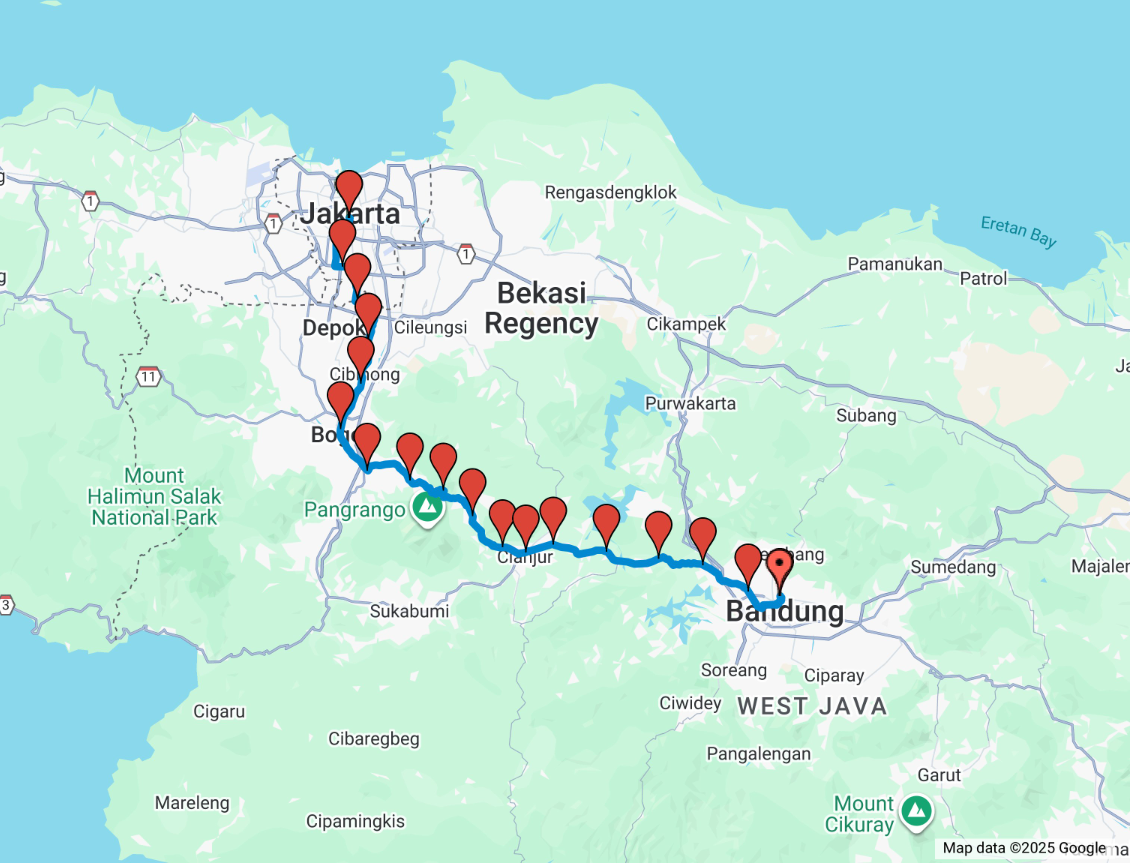
\includegraphics[width=\textwidth]{images/rute2025.png}
    \caption{Rute ITB Ultra-Marathon 2025 }
    \label{fig:rute-itb-ultra-2025}
\end{figure}

Selain jaraknya yang ekstrem, ITB Ultra-Marathon juga terkenal dengan sistem \textit{relay}-nya. Sistem \textit{relay} ini berfungsi untuk mengakomodasi berbagai tingkat keahlian dan stamina peserta, sekaligus menyoroti pentingnya kerja sama tim serta strategi pembagian beban untuk berhasil mencapai garis \textit{finish}. Berikut ini merupakan pembagian kategori peserta pada ITB Ultra-Marathon.

\input{tables/kategori.tex}

Secara umum, kategori lomba pada ITB Ultra-Marathon dibagi menjadi dua jenis utama, yaitu Individu dan \textit{Relay}. Kategori \textit{Relay} menawarkan empat format berbeda yang didasarkan pada jumlah anggota tim, yaitu tim yang terdiri dari 2 orang, 4 orang, 8 orang, atau 16 orang. Pembagian total jarak tempuh 180 kilometer akan menyesuaikan secara proporsional dengan banyaknya anggota tim, memastikan setiap pelari dalam tim \textit{relay} menempuh jarak yang telah ditentukan.

Tidak hanya pelari, penyelenggaraan ITB Ultra-Marathon juga melibatkan panitia penyelenggara, tim support, dan penonton dari masing-masing peserta maraton. Maka dari itu, koordinasi menjadi tantangan tersendiri mengingat kegiatan berlangsung selama berjam-jam dengan rute yang panjang dan melibatkan banyak \textit{checkpoint}. Sistem pelacakan yang efektif menjadi kebutuhan penting untuk mendukung koordinasi, memastikan keselamatan peserta, dan memberikan informasi \textit{real-time} kepada seluruh pihak yang terlibat selama maraton berlangsung.

\section{Sistem \textit{tracker} dalam Perlombaan Lari Jarak Jauh}
\textit{Tracker} atau sistem pelacakan adalah teknologi yang digunakan untuk memantau dan merekam posisi, pergerakan, atau status suatu objek secara \textit{real-time} atau periodik. Dalam konteks ajang \textit{ultra-marathon}, sistem pelacakan memegang peranan penting untuk memastikan keselamatan peserta, pemantauan performa, dan koordinasi panitia. Sistem ini berfungsi untuk memantau lokasi pelari, kecepatan, jarak tempuh, dan metrik performa lainnya \cite{baca2009ubiquitous}.

Selain aspek teknis, penggunaan \textit{tracker} juga mempengaruhi pengalaman psikologis pelari. Dengan akses \textit{real-time} terhadap data performa mereka, pelari dapat menyesuaikan strategi selama lomba, mengatur ritme, dan menetapkan target yang realistis \cite{karahanouglu2021sports}. Data ini tidak hanya membantu pelari dalam perencanaan fisik, tetapi juga meningkatkan motivasi dan rasa kontrol terhadap pencapaian mereka. Lebih jauh, sistem pelacakan memungkinkan panitia untuk melakukan intervensi cepat jika terjadi kondisi darurat, sehingga keselamatan peserta tetap terjaga. Dengan demikian, \textit{tracker} berperan ganda, yakni sebagai alat evaluasi performa sekaligus penunjang keselamatan dan pengalaman psikologis peserta.

Sistem \textit{tracking} modern umumnya memanfaatkan teknologi GPS (\textit{Global Positioning System}) yang terintegrasi dengan perangkat \textit{mobile} untuk memberikan data lokasi dengan akurasi tinggi. GPS adalah sistem navigasi berbasis satelit yang dikembangkan oleh Departemen Pertahanan Amerika Serikat dan kini telah menjadi teknologi global yang dapat diakses secara bebas untuk keperluan sipil \cite{el2002introduction}. Sistem ini bekerja dengan memanfaatkan jaringan satelit yang mengorbit bumi untuk menentukan posisi geografis suatu objek berdasarkan perhitungan trilaterasi dari sinyal yang diterima oleh \textit{receiver} GPS \cite{kaplan2017understanding}.

Dalam penerapannya untuk \textit{event ultra-marathon}, GPS \textit{tracking} menghadapi tantangan khusus, seperti konsumsi baterai yang tinggi untuk pemantauan kontinu selama berjam-jam, variasi akurasi di berbagai medan (trail, hutan, pegunungan), serta ketergantungan pada jaringan data untuk transmisi lokasi secara \textit{real-time} \cite{gilgen2019rr}. Dengan memahami karakteristik dan keterbatasan teknologi GPS, pengembangan aplikasi \textit{tracker} dapat dirancang dengan strategi mitigasi yang tepat guna memastikan reliabilitas sistem selama \textit{event} berlangsung.

\section{Konsep Dasar \textit{Front-End Development}}
\textit{Front-end development} adalah proses pengembangan bagian aplikasi yang berinteraksi langsung dengan pengguna melalui antarmuka visual (\textit{user interface}). \textit{Front-end} mencakup semua elemen visual, interaksi, dan logika presentasi yang ditampilkan di sisi klien \cite{bollini2017beautiful}. Dalam konteks aplikasi web maupun \textit{mobile}, \textit{front-end} bertanggung jawab untuk menampilkan data, menerima input pengguna, dan berkomunikasi dengan \textit{back-end} melalui API untuk pertukaran data. Berbeda dengan \textit{back-end} yang mengelola logika bisnis dan basis data di sisi server, \textit{front-end} sepenuhnya berorientasi pada pengalaman pengguna dan bagaimana informasi dikomunikasikan secara visual dan interaktif.

Komponen utama dalam \textit{front-end development} meliputi struktur konten menggunakan HTML atau \textit{framework} berbasis komponen (\textit{component-based}), \textit{styling} dan tata letak menggunakan CSS atau \textit{utility framework}, logika interaksi menggunakan JavaScript atau \textit{framework} modern seperti React, Vue, atau Angular, serta integrasi dengan \textit{back-end} melalui REST API maupun GraphQL \cite{osmani2023learning}. Masing-masing komponen ini bekerja secara sinergis: HTML mendefinisikan struktur semantik konten, CSS mengatur presentasi visualnya, sedangkan JavaScript menambahkan lapisan interaktivitas dan pengelolaan data dinamis yang membuat aplikasi dapat merespons perubahan secara \textit{real-time} tanpa perlu memuat ulang halaman.

\textit{Front-end} yang baik harus memenuhi sejumlah prinsip kualitas yang mempengaruhi baik kegunaan maupun jangkauan aplikasi. Pertama, \textit{responsiveness}, yaitu kemampuan antarmuka untuk beradaptasi secara fleksibel terhadap berbagai ukuran layar, mulai dari perangkat \textit{desktop} hingga \textit{smartphone}, sehingga pengguna mendapatkan pengalaman yang konsisten di berbagai perangkat \cite{marcotte2017responsive}. Kedua, \textit{accessibility}, yaitu kemampuan aplikasi untuk dapat diakses dan digunakan oleh semua pengguna tanpa terkecuali, termasuk penyandang disabilitas visual maupun motorik, sesuai dengan prinsip \textit{human-centred design} yang menekankan pentingnya merancang sistem yang inklusif bagi seluruh pengguna \cite{maguire2001methods}. Ketiga, \textit{performance}, yang berkaitan dengan kecepatan pemuatan dan respons aplikasi terhadap interaksi pengguna. Penelitian menunjukkan bahwa pengguna web memiliki toleransi waktu tunggu yang sangat terbatas, dengan tingkat intoleransi yang mulai muncul pada rentang 12 detik waktu respons, sehingga performa pemuatan halaman secara langsung mempengaruhi kepuasan dan niat pengguna untuk kembali menggunakan aplikasi \cite{nah2004study}.

Dalam pengembangan aplikasi \textit{tracker} untuk ITB Ultra-Marathon, \textit{front-end} memiliki peran yang sangat krusial. Aplikasi ini harus mampu menyajikan data lokasi peserta secara \textit{real-time} melalui peta interaktif, menampilkan metrik performa pelari seperti kecepatan dan jarak tempuh, serta menyediakan antarmuka untuk manajemen tim dan notifikasi. Tantangan khususnya terletak pada kondisi lapangan yang dinamis — pengguna mengakses aplikasi dari berbagai perangkat dengan koneksi jaringan yang bervariasi, sehingga kualitas \textit{front-end} secara langsung mempengaruhi efektivitas koordinasi dan pemantauan selama \textit{event} berlangsung. Oleh karena itu, subbab berikut membahas empat aspek teknis yang menjadi landasan pengembangan \textit{front-end} pada sistem ini, yaitu GIS dan visualisasi peta, desain UI/UX, \textit{state management}, serta teknologi integrasi data.

\subsection{\textit{Geographic Information System (GIS)} dan Visualisasi Peta}
\textit{Geographic Information System} (GIS) adalah sistem berbasis komputer yang dirancang untuk mengumpulkan, menyimpan, mengelola, menganalisis, dan menampilkan data yang memiliki referensi geografis atau spasial \cite{longley2015geographic}. GIS mengintegrasikan berbagai lapisan informasi ke dalam satu representasi peta yang koheren, sehingga memungkinkan pengguna untuk memahami pola, hubungan, dan konteks spasial dari suatu data secara intuitif. Dalam dekade terakhir, GIS telah berkembang melampaui aplikasi tradisional di bidang kartografi dan perencanaan wilayah, merambah ke berbagai domain seperti manajemen bencana, kesehatan publik, transportasi, hingga olahraga.

Komponen utama dalam GIS terdiri atas data spasial (berupa vektor maupun raster), data atribut yang melekat pada entitas geografis, serta perangkat lunak pengolah yang mampu melakukan operasi spasial seperti \textit{overlay}, \textit{buffering}, dan analisis jaringan \cite{burrough2015principles}. Data vektor merepresentasikan fitur geografis dalam bentuk titik, garis, dan poligon, sedangkan data raster merepresentasikan permukaan bumi sebagai kisi piksel dengan nilai numerik. Kedua format ini sering digunakan secara komplementer bergantung pada kebutuhan analisis dan resolusi data yang tersedia.

Dalam konteks pengembangan aplikasi berbasis web, teknologi GIS telah berevolusi menjadi \textit{Web GIS} yang memungkinkan visualisasi dan interaksi peta secara langsung melalui peramban tanpa memerlukan instalasi perangkat lunak khusus \cite{fu2010web}. Pustaka JavaScript seperti Leaflet.js dan Mapbox GL JS menjadi pilihan populer untuk implementasi \textit{Web GIS} karena menawarkan antarmuka pemrograman yang ringan, fleksibel, dan mudah diintegrasikan dengan \textit{framework} pengembangan \textit{front-end} modern. Leaflet.js secara khusus mendukung penambahan lapisan peta interaktif, penanda lokasi, serta \textit{polyline} untuk merepresentasikan jalur atau rute secara dinamis.

Visualisasi peta dalam konteks perlombaan lari jarak jauh memerlukan kemampuan untuk menampilkan jalur lintasan, posisi peserta secara \textit{real-time}, serta titik-titik penting seperti pos pemeriksaan (\textit{checkpoint}) dan lokasi darurat. Tantangan dalam visualisasi ini mencakup sinkronisasi data lokasi yang terus berubah, pengelolaan performa \textit{rendering} untuk banyak objek bergerak secara bersamaan, serta adaptasi tampilan terhadap berbagai ukuran layar perangkat \cite{maceachren2001research}. Oleh karena itu, desain arsitektur sistem visualisasi perlu mempertimbangkan strategi pembaruan data yang efisien agar latensi dapat ditekan seminimal mungkin.

\subsection{\textit{User Interface (UI)} dan \textit{User Experience (UX)}}
\textit{User Interface} (UI) merujuk pada elemen visual dan interaktif yang menjadi titik kontak antara pengguna dengan sebuah sistem digital, mencakup tata letak, tipografi, warna, ikon, dan komponen interaktif lainnya \cite{galitz2007essential}. Sementara itu, \textit{User Experience} (UX) adalah konsep yang lebih luas, meliputi keseluruhan persepsi, respons emosional, dan kepuasan pengguna yang timbul dari interaksi mereka dengan produk atau layanan tersebut \cite{maguire2001methods}. Meskipun keduanya saling berkaitan erat, UI berfokus pada aspek tampilan (\textit{look}) sedangkan UX berfokus pada aspek pengalaman (\textit{feel}) secara menyeluruh.

Desain UI yang baik mengedepankan prinsip keterbacaan, konsistensi visual, dan hierarki informasi yang jelas agar pengguna dapat menavigasi antarmuka secara intuitif tanpa beban kognitif yang berlebihan \cite{nielsen1994usability}. Dalam konteks aplikasi pelacakan \textit{real-time} seperti sistem pemantauan ultra-marathon, desain UI perlu mengakomodasi kepadatan informasi yang tinggi, seperti data posisi, kecepatan, dan status peserta, sekaligus tetap mempertahankan keterbacaan di berbagai kondisi penggunaan, termasuk pada layar perangkat \textit{mobile}.

Dari sisi UX, pendekatan \textit{user-centred design} (UCD) menekankan pentingnya melibatkan pengguna akhir secara aktif dalam setiap tahap proses perancangan, mulai dari identifikasi kebutuhan, pembuatan prototipe, hingga pengujian usabilitas \cite{maguire2001methods}. Penerapan prinsip UCD memastikan bahwa fitur-fitur yang dikembangkan benar-benar relevan dengan kebutuhan nyata pengguna, baik itu panitia yang membutuhkan \textit{dashboard} pemantauan komprehensif, maupun penonton yang memerlukan antarmuka sederhana untuk mengikuti posisi peserta tertentu.


\subsection{\textit{State Management} dalam Aplikasi \textit{Front-End}}
\textit{State management} adalah mekanisme untuk mengelola dan mendistribusikan data dinamis (\textit{state}) di dalam sebuah aplikasi \textit{front-end}, sehingga setiap komponen antarmuka dapat merespons perubahan data secara konsisten dan terkoordinasi \cite{lazuardy2022modern}. Dalam aplikasi berbasis komponen seperti yang dibangun dengan React atau Vue.js, \textit{state} dapat bersifat lokal (hanya relevan untuk satu komponen) atau global (dibagikan ke banyak komponen sekaligus). Pengelolaan \textit{state} yang tidak tepat dapat menimbulkan inkonsistensi tampilan dan menyulitkan proses \textit{debugging}, terutama pada aplikasi dengan aliran data yang kompleks.

Untuk aplikasi berskala besar, berbagai solusi \textit{state management} telah dikembangkan guna menyediakan sumber kebenaran tunggal (\textit{single source of truth}) bagi seluruh komponen aplikasi. Redux, misalnya, menerapkan pola arsitektur \textit{flux} yang mengharuskan setiap perubahan \textit{state} dilakukan melalui aksi (\textit{action}) yang terdefinisi secara eksplisit, sehingga aliran data menjadi lebih mudah dilacak dan diuji \cite{lazuardy2022modern}. Alternatif yang lebih ringan seperti Zustand atau React Context API juga semakin banyak digunakan untuk kebutuhan yang tidak memerlukan kompleksitas penuh dari Redux.

Dalam konteks aplikasi pelacakan \textit{real-time}, \textit{state management} memegang peranan krusial karena data posisi peserta diperbarui secara kontinu dari server. Setiap pembaruan data harus segera dipropagasikan ke seluruh komponen yang relevan, seperti peta, tabel peringkat, dan panel statistik, tanpa menyebabkan \textit{re-render} yang tidak perlu sehingga performa aplikasi tetap optimal. Oleh karena itu, pemilihan strategi \textit{state management} yang tepat perlu mempertimbangkan frekuensi pembaruan data, jumlah komponen yang bergantung pada \textit{state} tersebut, serta kebutuhan persistensi data di sisi klien \cite{lazuardy2022modern}.

\subsection{Teknologi Integrasi Data}
Integrasi data dalam aplikasi \textit{front-end} merujuk pada mekanisme yang digunakan untuk menghubungkan antarmuka pengguna dengan sumber data eksternal, seperti server \textit{back-end}, basis data, maupun layanan pihak ketiga \cite{richardson2008restful}. Terdapat beberapa paradigma komunikasi yang umum digunakan, masing-masing dengan karakteristik dan kasus penggunaan yang berbeda, di antaranya REST API, GraphQL, dan WebSocket.

REST (\textit{Representational State Transfer}) adalah arsitektur komunikasi berbasis HTTP yang paling banyak digunakan dalam pengembangan aplikasi web modern. REST menggunakan metode HTTP standar seperti GET, POST, PUT, dan DELETE untuk melakukan operasi terhadap sumber daya yang direpresentasikan dalam format JSON atau XML \cite{fielding2000architectural}. Keunggulan REST terletak pada kesederhanaan, skalabilitas, dan dukungan luas dari berbagai \textit{framework} dan \textit{library}, menjadikannya pilihan utama untuk komunikasi data yang bersifat permintaan-respons (\textit{request-response}).

Namun, untuk kebutuhan data \textit{real-time} seperti pembaruan posisi peserta secara kontinu dalam sistem pelacakan ultra-marathon, REST API memiliki keterbatasan karena bersifat \textit{stateless} dan mengharuskan klien melakukan \textit{polling} secara periodik. Sebagai solusi, protokol WebSocket memungkinkan komunikasi dua arah (\textit{full-duplex}) yang persisten antara klien dan server, sehingga server dapat mengirimkan data ke klien kapan saja tanpa perlu menunggu permintaan \cite{pimentel2012websocket}. Pendekatan ini secara signifikan mengurangi latensi dan beban jaringan dibandingkan dengan teknik \textit{polling} konvensional, menjadikannya pilihan yang lebih tepat untuk aplikasi yang memerlukan pembaruan data dengan frekuensi tinggi.

Selain WebSocket, teknologi \textit{Server-Sent Events} (SSE) juga dapat menjadi alternatif untuk komunikasi satu arah dari server ke klien. SSE lebih sederhana untuk diimplementasikan dibandingkan WebSocket dan didukung secara natif oleh peramban modern, namun hanya mendukung aliran data dari server ke klien saja \cite{pimentel2012websocket}. Pemilihan antara WebSocket, SSE, atau REST \textit{polling} pada akhirnya bergantung pada kebutuhan spesifik aplikasi, termasuk frekuensi pembaruan data, kebutuhan komunikasi dua arah, dan kompleksitas infrastruktur yang dapat ditanggung oleh tim pengembang.


% \section{Tentang Studi Literatur}
% Studi literatur biasanya berisi tentang tinjauan pustaka, landasan teori, dan penelitian-penelitian terdahulu yang relevan dengan topik tugas akhir yang dikerjakan.
% Dalam subbab ini, penulis diharapkan dapat menjelaskan:
% \begin{enumerate}
%   \item Landasan teori yang diperoleh dari literatur yang akan digunakan untuk menyelesaikan persoalan TA;
%   \item Pengetahuan tentang kasus yang akan dikaji; dan
%   \item Penelitian atau solusi terkait untuk mengetahui posisi persoalan dan berbagai solusi yang memungkinkan untuk diterapkan berdasarkan hasil studi literatur ini.
% \end{enumerate}
% Jadi, studi literatur ini bukan sekadar rangkuman dari berbagai sumber referensi, tetapi harus diolah dan disajikan secara sistematis sehingga dapat memberikan gambaran yang jelas tentang landasan teori dan penelitian-penelitian terdahulu yang relevan dengan topik tugas akhir.

% Penulisan studi literatur yang baik dimulai dari penjelasan tentang kasus yang akan dikaji, kemudian diikuti dengan penjelasan tentang teori-teori yang relevan, dan diakhiri dengan tinjauan terhadap penelitian-penelitian terdahulu yang berkaitan dengan topik tugas akhir.
% Misalnya, jika topik tugas akhir adalah tentang masalah klasifikasi biji kopi berdasarkan citra kopi, 
% penulis dapat memulai dengan menjelaskan terlebih dahulu tentang karakteristik biji kopi, masalah dalam melakukan klasifikasi biji kopi, 
% kemudian menjelaskan tentang berbagai metode berbasis komputer yang dapat digunakan untuk mengklasifikasikan biji kopi berdasarkan citranya, 
% metode terbaik yang memungkinkan untuk diterapkan, teori-teori dasar tentang metode tersebut, dan diakhiri dengan tinjauan terhadap penelitian-penelitian terdahulu yang menggunakan metode untuk klasifikasi citra.

% Dalam studi literatur, biasanya banyak penjelasan tentang teori-teori yang disertai dengan rumus atau persamaan matematika, gambar, tabel, algoritma, pseudocode, atau kode program.
% Oleh karena itu, pada subbab berikut akan dijelaskan beberapa hal teknis terkait format penulisan dokumen tugas akhir.

% \section{Format Penulisan Gambar, Tabel, Rumus, dan Kode Program}
% Berikut adalah beberapa contoh penulisan gambar, tabel, rumus, dan kode program yang sesuai dengan format penulisan tugas akhir.
% \subsection{Penulisan Gambar}
% Contoh gambar dapat dilihat pada Gambar \ref{fig:jaringan} dan Gambar \ref{fig:jaringan2}.
% Secara vertikal, gambar biasanya diletakkan di bagian atas halaman (\textit{top}) atau di bagian bawah halaman (\textit{bottom}).
% Gambar tidak harus diletakkan tepat di tempat gambar tersebut disebutkan pertama kali dalam teks,
% tetapi dapat diletakkan di halaman berikutnya jika tidak muat di halaman yang sama. Pada contoh ini, kedua gambar diletakkan di bagian atas halaman 
% menggunakan opsi \texttt{[t]} pada lingkungan \texttt{figure}, namun pada halaman yang berbeda, meskipun disebutkan di halaman yang sama akibat ruang yang terbatas. 

% Penyebutan judul gambar dalam teks menggunakan perintah \texttt{ref}, misalnya Gambar \texttt{\\ref\{fig:jaringan\}}.
% Gunakan huruf kapital pada kata "Gambar" saat menyebutkan gambar dalam teks.

% \begin{figure}[t] % pilihan opsi yang disarankan: t = top, b = bottom, h = here
%   \caption{Contoh peletakan gambar di bagian atas halaman} 
% 	\label{fig:jaringan}
%     	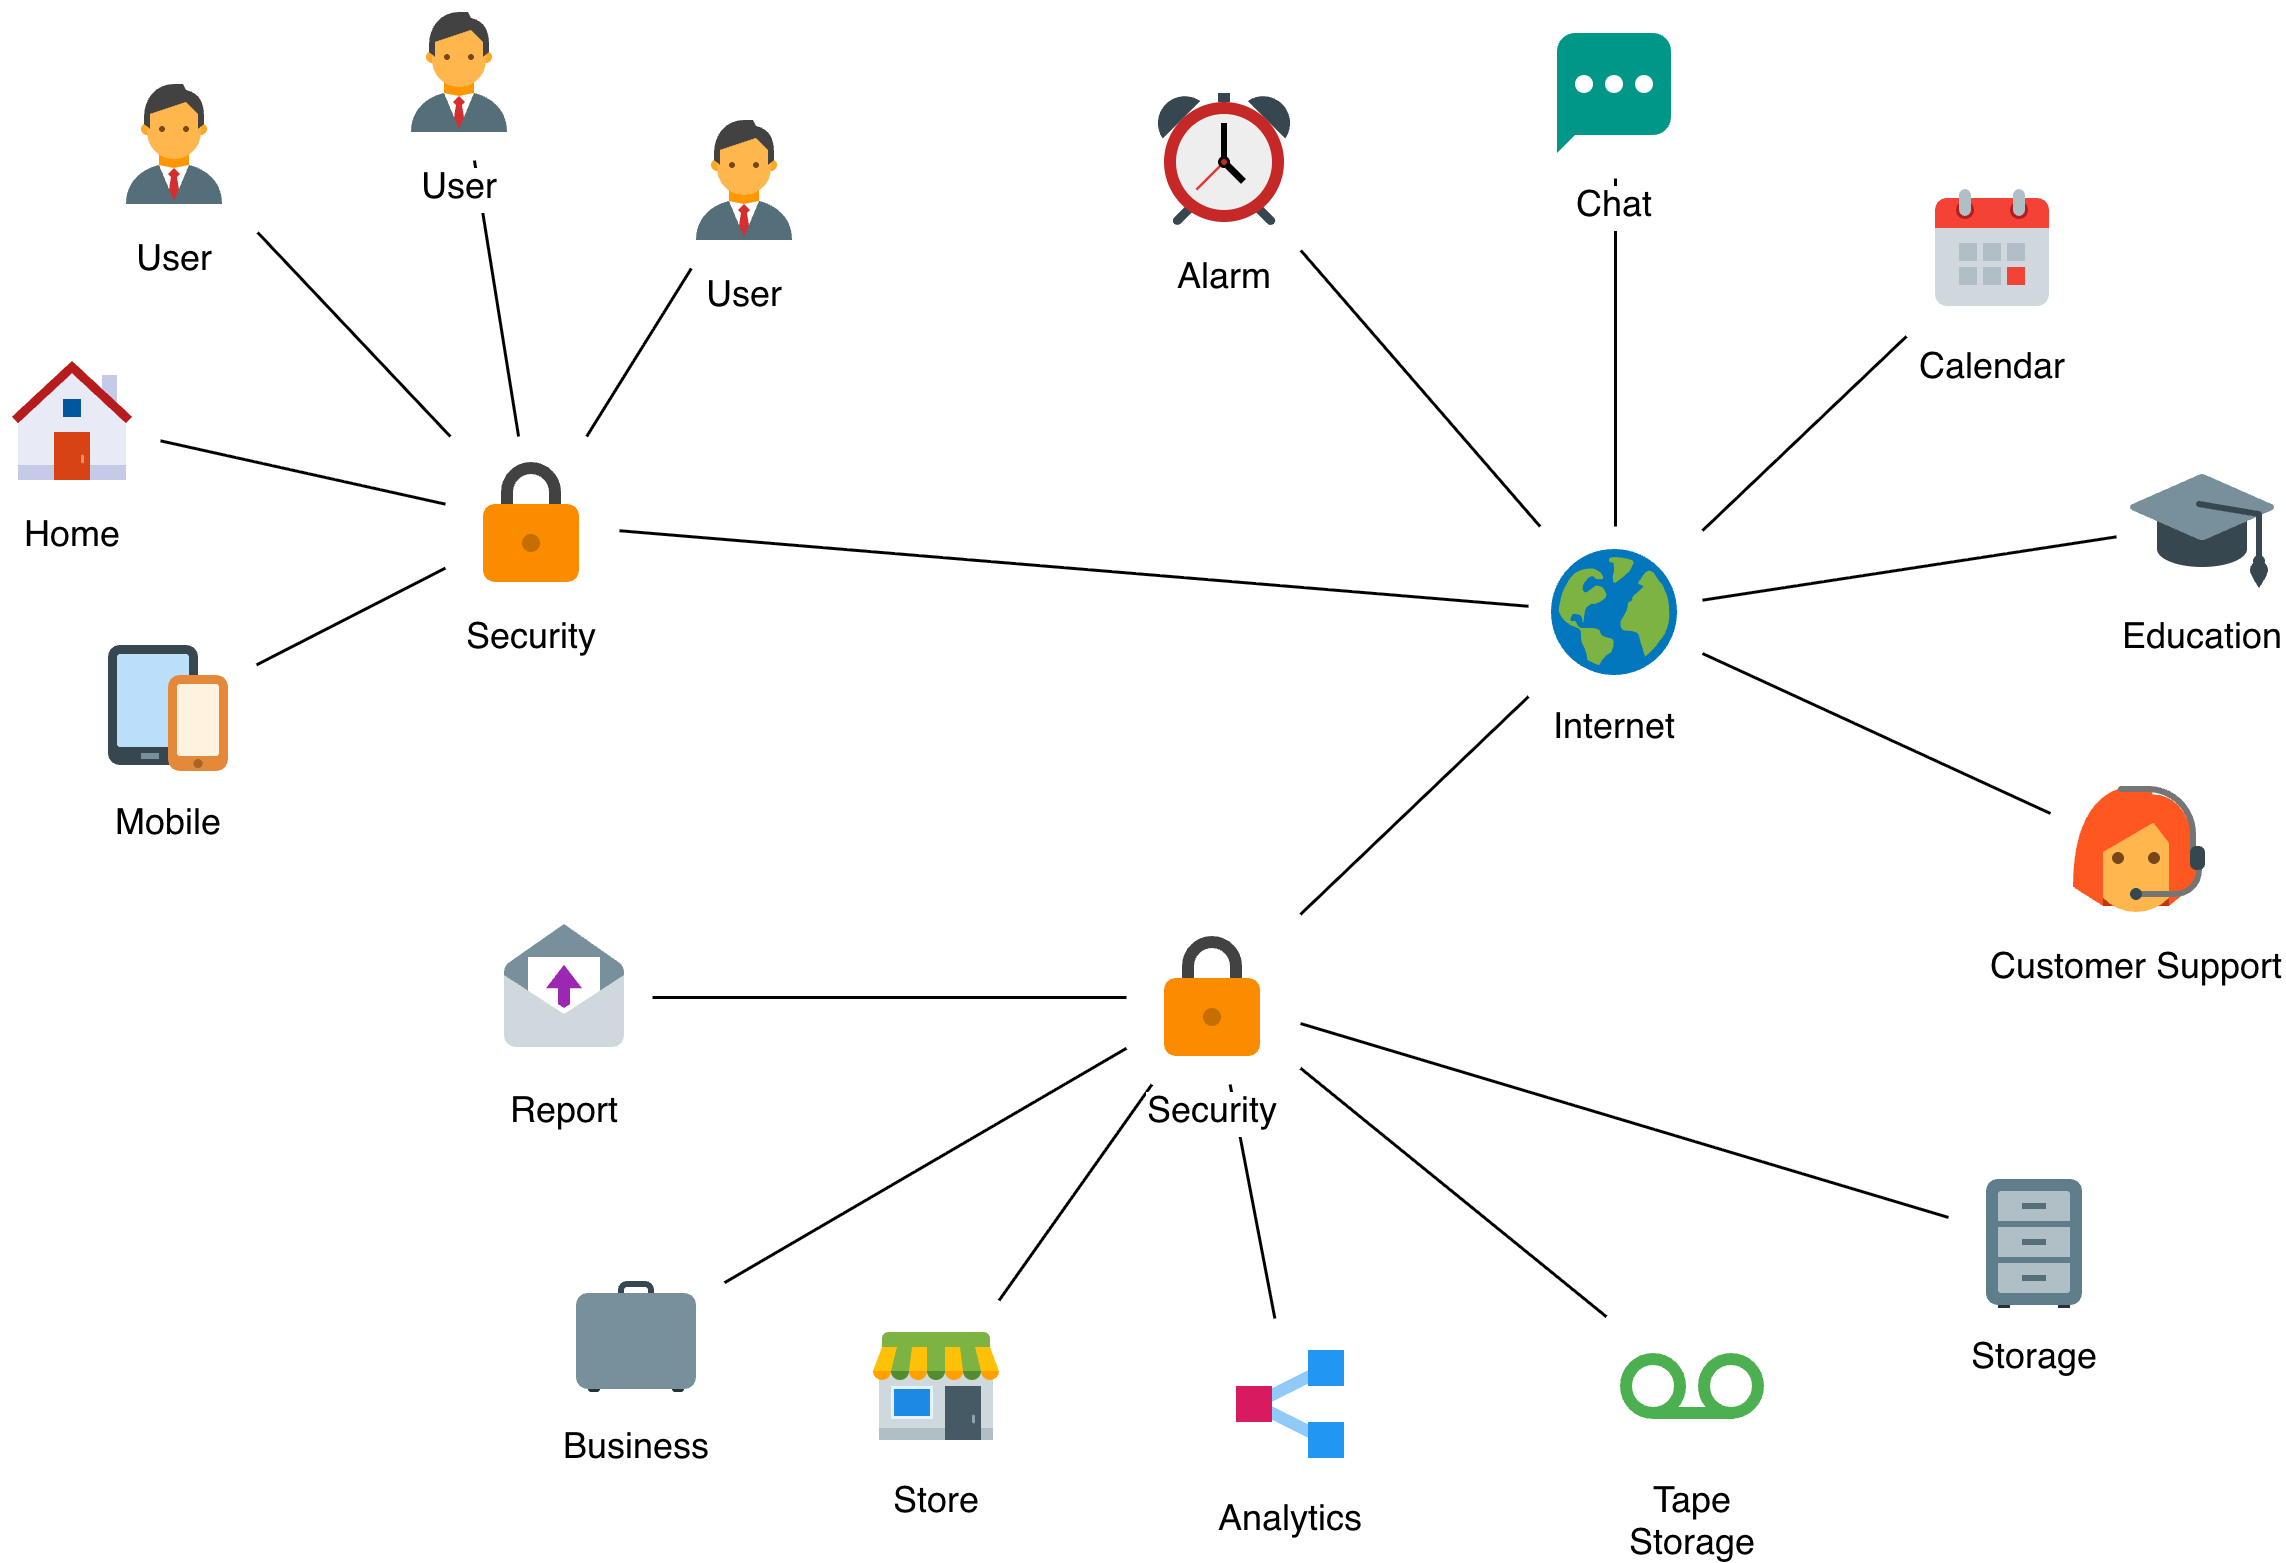
\includegraphics[width=0.7\textwidth]{images/gambar1.png}
% \end{figure}

% Gambar, grafik, atau ilustrasi harus memiliki keterangan atau judul (\textit{caption}) yang menjelaskan isi gambar tersebut. 
% Secara horisontal, gambar dan judulnya diposisikan di tengah. Nomor gambar tidak diakhiri tanda baca.
% Judul gambar diletakkan di bawah gambar dan ditulis dengan huruf kecil kecuali huruf pertama pada kalimat judul. 
% Kalimat judul yang panjang dapat ditulis dalam beberapa baris seperti pada Gambar \ref{fig:jaringan2}.

% Ukuran gambar yang ditampilkan dapat diatur dengan mengubah nilai \textit{width} dalam sintaks \textit{includegraphics}. 
% Gambar \ref{fig:jaringan} memiliki lebar 70\% dari lebar teks, sedangkan Gambar \ref{fig:jaringan2} memiliki lebar 90\% dari lebar teks.
 

% \begin{figure}[t] 
%   \caption{Contoh peletakan gambar dengan judul yang panjang sehingga ditulis dalam beberapa baris} 
% 	\label{fig:jaringan2}
%     	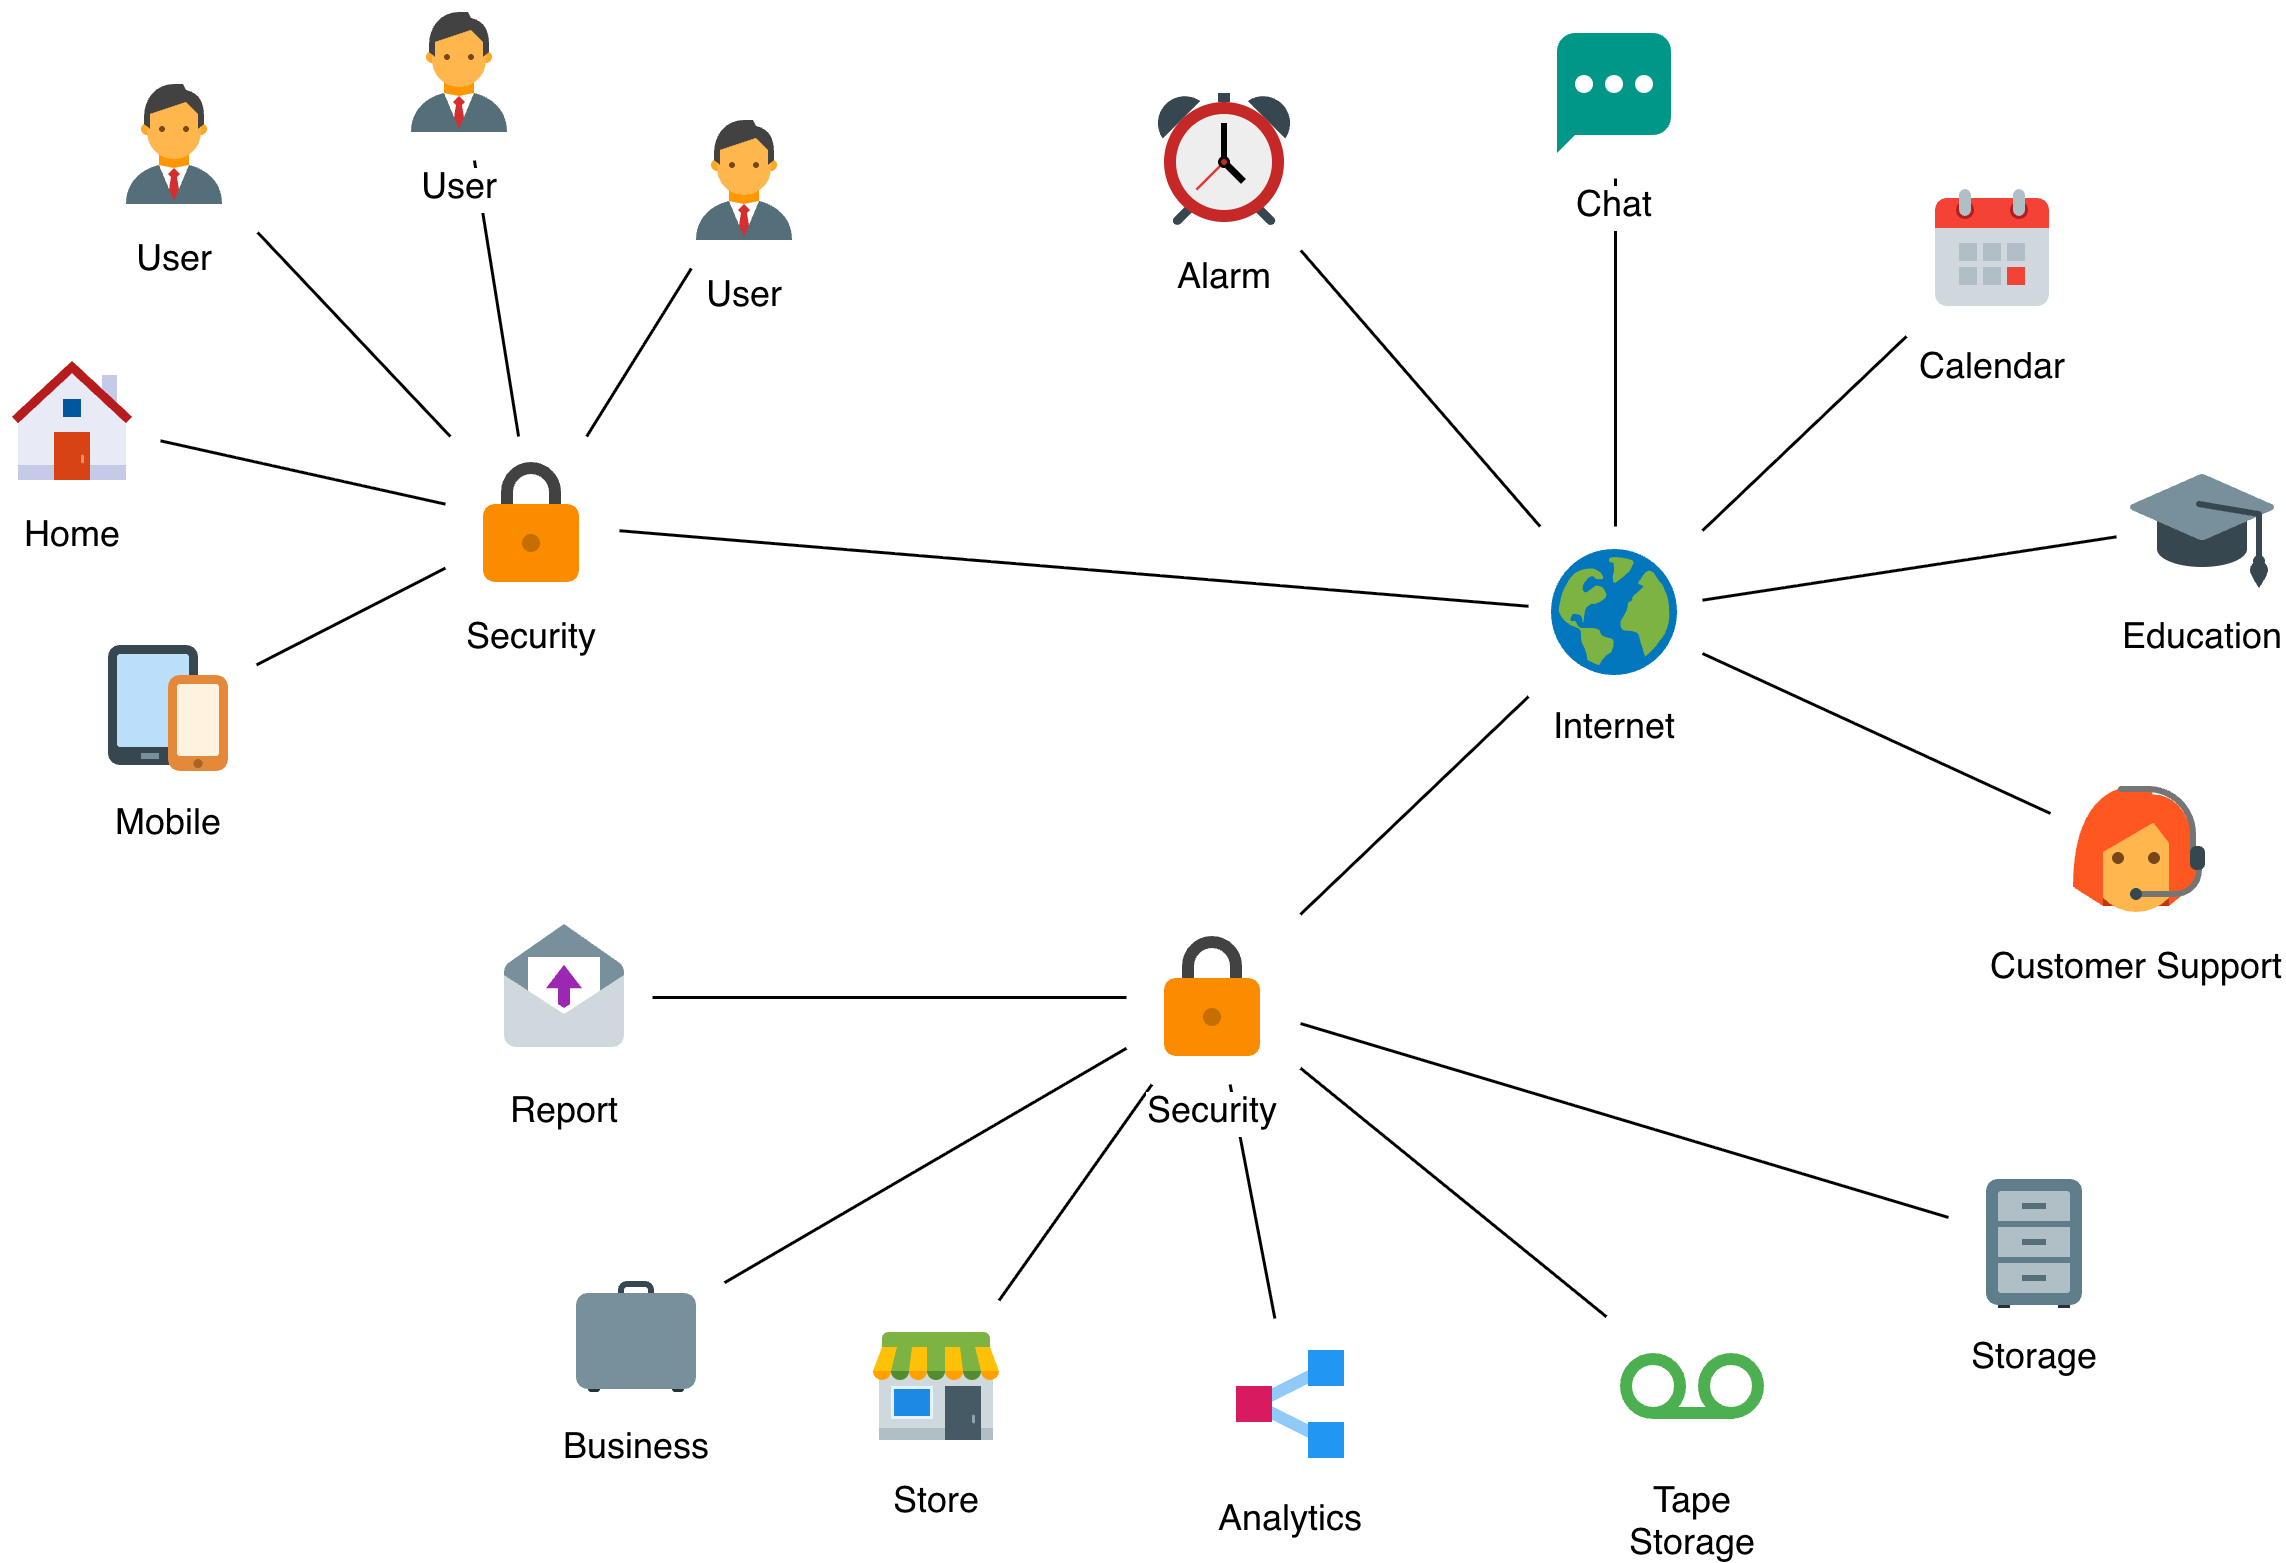
\includegraphics[width=0.9\textwidth]{images/gambar1.png}
% \end{figure}

% Pastikan gambar yang digunakan memiliki resolusi yang cukup tinggi agar tidak pecah atau buram saat dicetak. 
% Gambar umumnya tidak tajam dan tulisan tidak jelas atau kabur jika gambar tersebut:
% \begin{enumerate}[a.]
%   \item diperoleh dari hasil cropping pada suatu halaman buku atau situs web;
%   \item hasil pembesaran gambar yang gambar aslinya sebenarnya berukuran kecil; atau
%   \item disimpan dalam resolusi kecil
% \end{enumerate}
% Ketidakjelasan gambar ini dapat dilihat pada garis-garis diagram yang tidak tegas dan tulisan-tulisan dalam gambar yang tampak kabur dan kurang jelas terbaca.

% Untuk mendapatkan gambar yang tidak kabur (\textit{blur}), langkah-langkah berikut dapat digunakan:
% \begin{enumerate}[(a)]
% \item Hindari \textit{screenshot}. Gambar yang didapat di suatu pustaka atau referensi sebaiknya digambar ulang (tidak perlu sama persis), misalnya menggunakan PowerPoint, Canva, Figma, draw.io, atau yang lainnya.
% \item Jika diagram atau ilustrasi digambar menggunakan draw.io, saat gambar disimpan ke format PNG atau JPG (\textit{export as}), lakukan \textit{zoom} ke minimal 300\% (\textit{the default value is} 100\%). 
% \item Jika diagram digambar dengan menggunakan \texttt{PowerPoint} atau aplikasi yang mengolah gambar vektor lainnya, gambar dapat langsung disimpan asalkan resolusinya tinggi.
% \end{enumerate}

% \subsection{Penulisan Tabel}
% Format penulisan tabel hampir sama dengan format penulisan gambar. Bedanya adalah judul tabel diletakkan di atas tabel, bukan di bawah tabel seperti pada gambar.
% Ada tabel yang bisa dimuat dalam satu halaman (tabel pendek) dan ada tabel panjang yang yang tidak muat dalam satu halaman. Kedua jenis tabel tersebut disusun dengan cara yang berbeda.
% Jika tabel sangat panjang, gunakan paket \textit{longtable} untuk membuat tabel yang dapat terpotong ke halaman berikutnya.
% Namun, jika tabel dapat dimuat dalam satu halaman, gunakan lingkungan \textit{table} biasa, tidak menggunakan \textit{longtable}.
% Usahakan tabel dapat ditulis dalam satu halaman, tidak terpotong ke halaman berikutnya, jika memungkinkan.

% \subsubsection{Penulisan Tabel Pendek}
% Contoh tabel pendek dapat dilihat pada Tabel \ref{tab:tabel1}, \ref{tab:tabel2}, dan \ref{tab:tabel3}. 
% Pada kedua table ini, tabel dan judulnya diposisikan di tengah secara horisontal dan 
% judul tabel diletakkan di atas tabel. Secara vertikal, tabel sebaiknya diletakkan di bagian atas atau bawah halaman.

% Penyebutan judul tabel dalam teks menggunakan perintah \texttt{ref}, misalnya Tabel \ref{tab:tabel1}.
% Gunakan huruf kapital pada kata "Tabel" saat menyebutkan tabel dalam teks.

% Tabel \ref{tab:tabel1} menggunakan paket \textit{tabularx} untuk mengatur lebar kolom secara fleksibel. 
% Selain itu, tabel ini juga menggunakan \textit{threeparttable} untuk menambahkan catatan kaki pada tabel 
% dan opsi \texttt{X} agar lebar kolom fleksibel menyesuaikan lebar tabel.
% Catatan kaki pada tabel ini menggunakan perintah \texttt{tablenotes} yang disediakan oleh paket \textit{threeparttable}.
% Catatan kaki pada tabel ini menggunakan perintah \texttt{\textbackslash footnotemark} dan \texttt{\textbackslash footnotetext} untuk menambahkan catatan kaki pada tabel.

% Tabel \ref{tab:tabel2} menggunakan format standar \texttt{| l | c | r |}. 
% Tabel \ref{tab:tabel3} menggunakan lebar kolom tetap (\textit{fixed width}) menggunakan \texttt{p\{width\}}.

% \begin{table} 
%   \centering
%     \begin{threeparttable}[t] % threeparttable agar bisa menambahkan catatan kaki pada tabel
%     \caption{Contoh tabel yang menggunakan \texttt{tabularx} untuk mengatur lebar kolom secara fleksibel. 
%     Selain itu, tabel ini juga menggunakan \texttt{threeparttable} untuk menambahkan catatan kaki pada tabel 
%     dan opsi \texttt{X} agar lebar kolom fleksibel menyesuaikan lebar tabel.}
%     \label{tab:tabel1}
%     \begin{tabularx}{0.6\textwidth}{| c | X| l | r @{}|} % @{} removes extra space at edges, X makes the column flexible width
% 	    \hline
% 	    No & Nama 	& Satuan 		& Harga \\
% 	    \hline
% 	    1 & Buku 	& Exemplar	& 25000 \\
% 	    2 & Komputer	& Unit		& 2500000 \\
% 	    3 & Pensil	& Buah		& 118900 \\
% 	    \hline
% 	  \end{tabularx} 
%     \begin{tablenotes}
%       \footnotesize
%       \item \footnotemark[1]Tabel harga berdasarkan data tahun 2023.
%       \item \footnotemark[2]Sumber: \url{https://www.example.com}
%     \end{tablenotes}
%   \end{threeparttable}
% \end{table}




% \begin{table}[t] % pilihan opsi yang disarankan: t = top, b = bottom, h = here
%   \caption{Tabel yang menggunakan format standar \texttt{| l | c | r |}}
%   \label{tab:tabel2}
% 	\begin{tabular}{ | l | c | r | }
% 	\hline
% 	Nama 	& Satuan 		& Harga \\
% 	\hline
% 	Buku 	& Exemplar	& 25000 \\
% 	Komputer	& Unit		& 2500000 \\
% 	Pensil	& Buah		& 118900 \\
% 	\hline
% 	\end{tabular}
% \end{table}


% \begin{table}[t] % pilihan opsi yang disarankan: t = top, b = bottom, h = here
%   \centering
%   \caption{Tabel yang lebar kolomnya dibuat tetap}
%   \label{tbl:tabel3}
% 	\begin{tabular}{  p{0.2\textwidth} | p{0.2\textwidth} | p{0.2\textwidth}  }
% 	\hline
% 	\textbf{Nama} 	& \textbf{Satuan} 		& \textbf{Harga} \\
% 	\hline
% 	Buku 	& Exemplar	& 25000 \\
% 	\emph{Komputer}	& Unit		& 2500000 \\
% 	Pensil	& Buah		& 118900 \\
% 	\hline
% 	\end{tabular}
% \end{table}

% % -- Example of importing table from external file --
% \subsubsection{Mengimpor Tabel dari Berkas Eksternal}

% Untuk kerapian penulisan, tabel tidak harus ditulis di dokumen utama. Sebagai contoh, Tabel \ref{tab:tabel4} diimpor dari berkas eksternal \texttt{table/tabel1.tex} menggunakan perintah \texttt{input}. 
% Dengan demikian, jika tabel tersebut perlu diubah, cukup mengubah pada berkas eksternal tersebut tanpa perlu mengubah pada berkas dokumen utama ini.

% \input tables/tabel1.tex


% % -- Example of long table --
% \subsubsection{Tabel yang Sangat Panjang}
% Jika tabel terlalu panjang sehingga tidak muat dalam satu halaman, gunakan paket 
% \textit{longtable} untuk membuat tabel yang dapat terpotong ke halaman berikutnya, 
% seperti pada Tabel \ref{tab:long}. 

% \input tables/longtable1.tex

% \subsection{Penulisan Rumus atau Persamaan Matematika Menggunakan {\LaTeX} dan Penomorannya}
% Contoh rumus matematika dapat ditulis seperti pada Persamaan \ref{eq:contoh1} di bawah ini. 
% Penomoran persamaan diletakkan di sebelah kanan, dan rumus ditulis dalam mode \textit{display math}.
% \begin{equation}
% E = mc^2
% \label{eq:contoh1}
% \end{equation}
% \eqcaption{Persamaan Pertama}

% Contoh lain penulisan rumus matematika yang lebih kompleks dapat ditulis seperti pada Persamaan \ref{eq:rumus2}.
% Perlu diperhatikan bahwa jika rumus terdiri dari beberapa baris, nomor persamaan hanya diletakkan pada baris terakhir, bukan pada setiap baris.
% \begin{align}
% f(x) &= ax^2 + bx + c \notag \\ % tidak menampilkan nomor pada baris ini
% f'(x) &= \frac{d}{dx}(ax^2 + bx + c) \notag \\ % tidak menampilkan nomor pada baris ini
%       &= 2ax + b 
%       \label{eq:rumus2} % nomor hanya muncul pada baris terakhir
% \end{align}
% \eqcaption{Persamaan Kedua}

% Jika rumus terlalu panjang untuk ditulis dalam satu baris, gunakan lingkungan \textit{multline} seperti pada Persamaan \ref{eq:rumus3} di bawah ini.
% \begin{multline} 
% y = a_0 + a_1x + a_2x^2 + a_3x^3 + a_4x^4 + a_5x^5 + a_6x^6 + a_7x^7 \\
%     + a_8x^8 + a_9x^9 + a_{10}x^{10} \label{eq:rumus3}
% \end{multline}
% \eqcaption{Persamaan Ketiga}

% Jika ada penurunan rumus yang terdiri dari beberapa baris, namun tidak memerlukan penomoran pada setiap baris dan tidak masuk di daftar persamaan, gunakan lingkungan \textit{align*}, misalnya:

% \begin{align*} 
% S &= \sum_{i=1}^{n} i^2 \\
%   &= 1^2 + 2^2 + 3^2 + \cdots + n^2 \\
%   &= \frac{n(n + 1)(2n + 1)}{6}
% \intertext{Contoh lainnya adalah rumus untuk mencari nilai rata-rata fungsi $f(x)$ pada interval $[p, q]$:}
% \bar{f} &= \frac{1}{q - p} \int_{p}^{q} f(x) \, dx \\
%         &= \frac{1}{q - p} \int_{p}^{q} (ax^2 + bx + c) \, dx \\
%         &= \frac{1}{q - p} \left[ \frac{a}{3}x^3 + \frac{b}{2}x^2 + cx \right]_p^q \\
%         &= \frac{a(q^3 - p^3)}{3(q - p)} + \frac{b(q^2 - p^2)}{2(q - p)} + c \label{eq:rumus4}
% \end{align*}




% \subsection{Penulisan Kode Program, \textit{Script} atau \textit{Pseudocode}}
% Contoh penulisan kode program, \textit{script}, atau \textit{pseudocode} dapat dilihat seperti pada \textit{listing} \ref{lst:binary_iter}. 
% Gunakan paket \textit{listings} untuk menulis \textit{source code} dalam bahasa pemrograman tertentu. 
% Kode seperti ini disebut dengan istilah \textit{listing}. 
% Kode program, \textit{script}, atau \textit{pseudocode} yang relatif pendek dapat ditulis di dalam
% dokumen utama. Namun, jika kode programnya sangat panjang, sebaiknya ditulis di berkas terpisah dan diletakkan di lampiran.

% \subsection{Penulisan Algoritma}
% Contoh penulisan algoritma dapat dilihat pada Algoritma \ref{alg:binary-search}. Ada beberapa paket yang dapat digunakan untuk menulis algoritma,
% misalnya \textit{algorithm2e}, \textit{algorithmic}, dan \textit{algpseudocode}. 
% Pada contoh ini digunakan paket \textit{algorithmic} untuk menulis algoritma. Setiap paket memiliki sintaks yang berbeda-beda.
% Oleh karena itu, pelajari dokumentasi paket yang digunakan untuk menulis algoritma.


% \input{listings/binary-search-python.tex}


% \input{algorithms/binary-search-alg.tex}



